\documentclass{Group_Templ}

\usepackage{fdsymbol}

\setlength{\parindent}{0pt}

\begin{document}

\section*{Exercise 5.3}
Let $f_{u,v}$ denote the water flow through edge $(u,v)\ \forall (u,v) \in \mathit{E}$.

We need to make sure that every sink can process more water than the amount which comes in:

\[
	\sum_{(u,s_i)\in \mathit{E}}f_{u,s_i}\le b_{s_i} \forall s_i \in S
\]

Furthermore the amount the edges can remove from a source needs to be at most the amount of incoming water:

\[
\sum_{(q_i,v)\in \mathit{E}}f_{q_i,v}\le a_{q_i} \forall q_i \in Q
\]

Our target function is to maximize the amount of water we can get rid of:

\[
\max \sum_{q_i\in Q}\sum_{(q_i,v)\in E} f_{q_i,v}
\]

Another important constraint is, that every middle vertex has to have an equal inflow and outflow:

\[
\sum_{(u,v)\in E}f_{u,v}=\sum_{(v,w)\in E}f_{v,w}\ \forall v\in V\setminus(Q\cup S)
\]

One thing missing is a cap for every channel so we cannot move more water through it than it is capable of.

\[
0 \le f_{u,v}\le C_{u,v}\ \forall(u,v)\in E
\]

So in short:

\begin{flalign*}
	\max \quad &\sum_{q_i \in Q}
	\sum_{(q_i,v)\in E} f_{q_i,v}\\
	\text{s.t.}\quad
	\sum_{(u,s_i)\in E} f_{u,s_i}
	&\leq b_{s_i}
	&&\forall s_i\in S,\\
	\sum_{(q_i,v)\in E} f_{q_i,v}
	&\leq a_{q_i}
	&&\forall q_i\in Q,\\
	\sum_{(u,v)\in E} f_{u,v}
	&= \sum_{(v,w)\in E} f_{v,w}
	&&\forall v\in V\setminus(Q\cup S),\\
	0\leq f_{u,v}
	&\leq C_{u,v}
	&&\forall (u,v)\in E.
\end{flalign*}


To survive the flood, the optimal objective value
must satisfy:
\[
z^* = \sum_{q_i \in Q} a_{q_i}
\]

If this condition is satisfied, all incoming water
can be transported to the sinks without exceeding
the channel capacities.


Potential savings can be identified by comparing
the capacity of each channel with its actual flow:
\[
C_{u,v} - f_{u,v}
\]

If this difference is positive, the channel has unused
capacity and could potentially be built with a
smaller capacity while preserving the computed flow.

\newpage

\section*{Exercise 5.4}

\begin{enumerate}
	\item 
	Restrictions:
	\begin{flalign}
		2x_1 + x_2 &\le 6 \\
		\frac{1}{2}x_1+x_2 &\le 3 \\
		x_1 &\ge 0 \\
		x_2 &\ge 0
	\end{flalign}
	
	This leads to following combinations: \newline
	$(1,2);(1,3);(1,4);(2,3);(2,4);(3,4)$
	
	\subsection*{(1,2)}
	\[2x_1+x_2\le 6 \Rightarrow 2x_1+x_2=6\]
	
	\[\frac{1}{2}x_1+x_2\le 3\quad \Rightarrow\quad \frac{1}{2}x_1+x_2=3\quad \Rightarrow\quad x_2=3-\frac{1}{2}x_1\]
	
	Substitute:
	\begin{flalign*}
		2x_1+(3-\frac{1}{2}x_1) &= 6 \\
		2x_1+3-\frac{1}{2}x_1 &=6 \\
		\frac{3}{2}x_1+3&=6 \\
		\frac{3}{2}x_1&=3 \\
		x_1 &=2
	\end{flalign*}
	
	Calculate $x_2$ for $x_1$:
	\begin{flalign*}
		x_2&=3-\frac{1}{2}*2	\\
		x_2&=2 \\
		\Rightarrow \text{Point}&:(2,2)
	\end{flalign*}
	
	Check:
	\setcounter{equation}{0}
	\begin{flalign}
		2\cdot2 + 2 &\le 6 \quad\checkmark \\
		\frac{1}{2}2+2 &\le 3 \quad\checkmark \\
		2 &\ge 0 \quad\checkmark \\
		2 &\ge 0 \quad\checkmark \\
		&\Rightarrow \text{Feasible solution} \notag
	\end{flalign}
	
	\subsection*{(1,3)}
	\[2x_1+x_2\le 6 \Rightarrow 2x_1+x_2=6\]
	
	\[x_1\ge 0\Rightarrow x_1=0\]
	
	Substitute:
	\begin{flalign*}
		2\cdot 0+x_2 &= 6 \\
		x_2 &=6 \\
		\Rightarrow \text{Point}&:(0,6)
	\end{flalign*}
	
	Check:
	\setcounter{equation}{0}
	\begin{flalign}
		2*0 + 6 &\le 6 \quad\checkmark \\
		\frac{1}{2}0+6 &\le 3 \quad\lightning \\
		&\Rightarrow \text{Infeasible solution} \notag
	\end{flalign}
	
	\subsection*{(1,4)}
	\[2x_1+x_2\le 6 \Rightarrow 2x_1+x_2=6\]
	
	\[x_2\ge 0\Rightarrow x_2=0\]
	
	Substitute:
	\begin{flalign*}
	2x_1+0 &= 6 \\
	x_1 &=3 \\
	\Rightarrow \text{Point}&:(3,0)
	\end{flalign*}
	
	Check:
	\setcounter{equation}{0}
	\begin{flalign}
	2\cdot3 + 0 &\le 6 \quad\checkmark \\
	\frac{1}{2}3+0 &\le 3 \quad\checkmark \\
	3 &\ge 0 \quad\checkmark \\
	0 &\ge 0 \quad\checkmark \\
	&\Rightarrow \text{Feasible solution} \notag
	\end{flalign}
	
	\subsection*{(2,3)}
	\[\frac{1}{2}x_1+x_2\le 3 \Rightarrow \frac{1}{2}x_1+x_2= 3\]
	
	\[x_1\ge 0\Rightarrow x_1=0\]
	
	Substitute:
	\begin{flalign*}
	\frac{1}{2}\cdot 0+x_2 &= 3 \\
	x_2 &=3 \\
	\Rightarrow \text{Point}&:(0,3)
	\end{flalign*}
	
	Check:
	\setcounter{equation}{0}
	\begin{flalign}
	2*0 + 3 &\le 6 \quad\checkmark \\
	\frac{1}{2}0+3 &\le 3 \quad\checkmark \\
	0 &\ge 0 \quad\checkmark \\
	3 &\ge 0 \quad\checkmark \\
	&\Rightarrow \text{Feasible solution} \notag
	\end{flalign}
	
	\subsection*{(2,4)}
	\[\frac{1}{2}x_1+x_2\le 3 \Rightarrow \frac{1}{2}x_1+x_2= 3\]
	
	\[x_2\ge 0\Rightarrow x_2=0\]
	
	Substitute:
	\begin{flalign*}
	\frac{1}{2}x_1+0 &= 3 \\
	x_1 &=6 \\
	\Rightarrow \text{Point}&:(6,0)
	\end{flalign*}
	
	Check:
	\setcounter{equation}{0}
	\begin{flalign}
	2*6 + 0 &\le 6 \quad\lightning \\
	&\Rightarrow \text{Infeasible solution} \notag
	\end{flalign}
	
	\subsection*{(3,4)}
	\[x_1\ge 0\Rightarrow x_1=0\]
	
	\[x_2\ge 0\Rightarrow x_2=0\]
	
	\begin{flalign*}
	\Rightarrow \text{Point}&:(0,0)
	\end{flalign*}
	
	Check:
	\setcounter{equation}{0}
	\begin{flalign}
	2*0 + 0 &\le 6 \quad\checkmark \\
	\frac{1}{2}0+0 &\le 3 \quad\checkmark \\
	0 &\ge 0 \quad\checkmark \\
	0 &\ge 0 \quad\checkmark \\
	&\Rightarrow \text{Feasible solution} \notag
	\end{flalign}
	
	Feasible solutions:
	\[
	\{(2,2);(3,0);(0,3);(0,0)\}
	\]
	
	Evaluating the objective function:
	\[
		\max{2x_1+x_2}
	\]
	\setcounter{equation}{0}
	\begin{flalign}
		2*2+2&=6 \\
		2*3+0&=6 \\
		2*0+3&=3 \\
		2*0+0&=0 \\
		\Rightarrow (2,2)&\text{ and }(3,0) \text{ are optimal solutions.} \notag
	\end{flalign}
	\newpage
	The graphical representation. One can clearly see, that all solutions on the edge between (3,0) and (2,2) are optimal solutions for this LP.
	
	\begin{minipage}[t]{\textwidth}
		\begin{figure}[H]
			\centering
			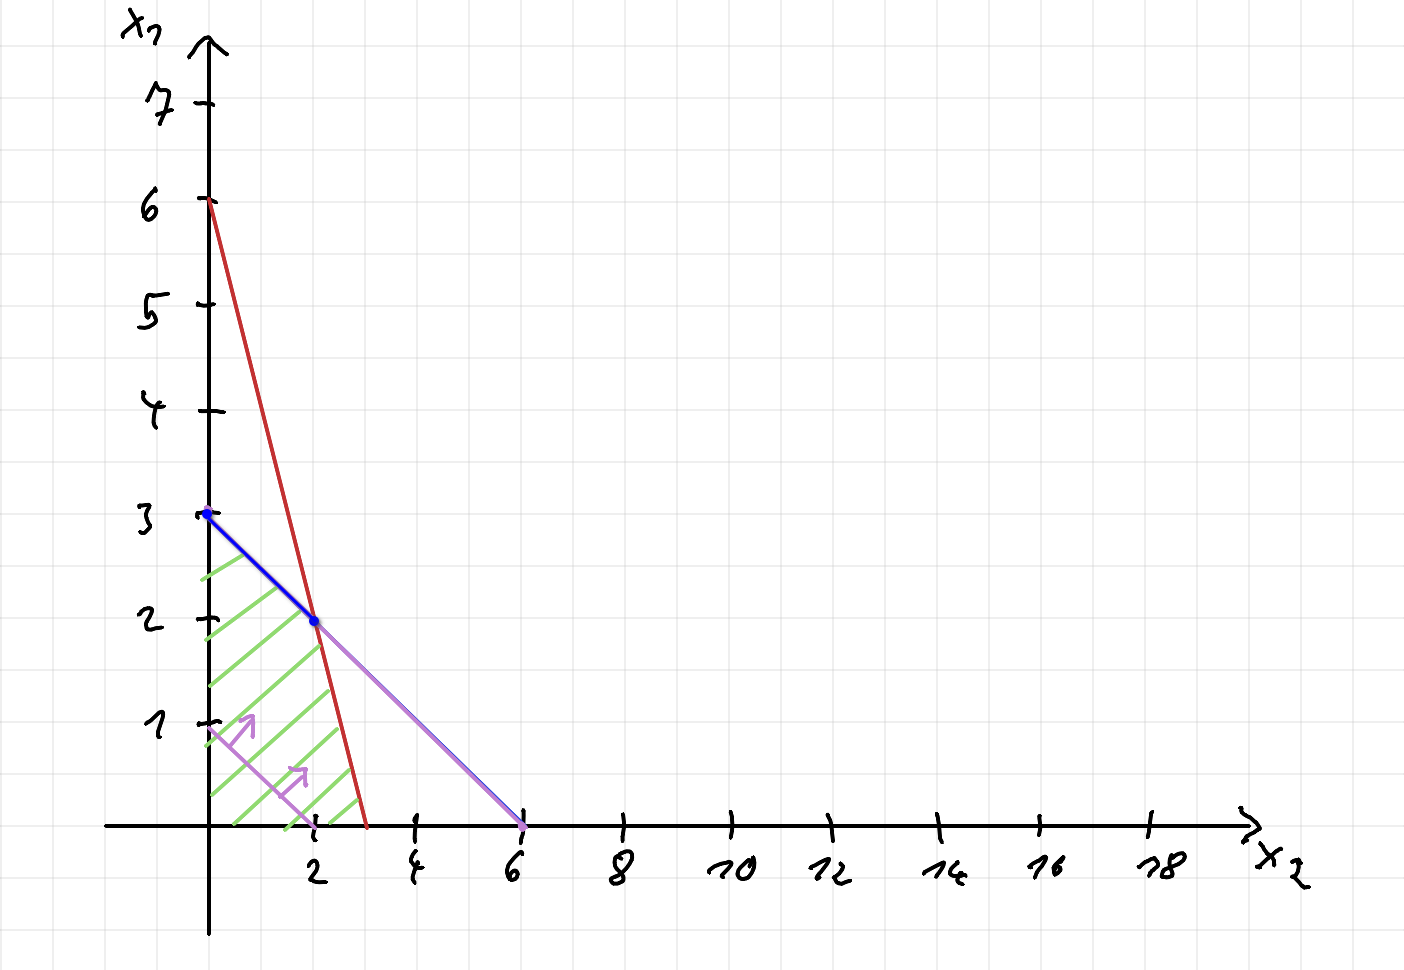
\includegraphics[width=0.8\textwidth]{5.4.1}
			\label{fig:label} % Optionales Label für Verweise
		\end{figure}
	\end{minipage}
	\item 
	\begin{flalign*}
		\max\quad &2x_1+x_2 \\
		\text{s.t.}\quad &2x_1+x_2\le 6 \\
		&\frac{1}{2}x_1+x_2\le 3 \\
		&x_1,x_2 \ge 0
	\end{flalign*}
	
	basic feasible solution: \[(x_1,x_2)=(0,0)\]
	
	Transform into slack form:
	\begin{flalign*}
		z &= \quad 2x_1 + x_2 \\
		x_3 &= 6 - 2x_1 - x_2 \\
		x_4 &= 3 - \frac{1}{2}x_1 - x_2 \\
		&x_1,x_2,x_3,x_4 \ge 0
	\end{flalign*}
	
	basic feasible solution: \[(x_1,x_2,x_3,x_4)=(0,0,6,3)\]
	
	\[\text{entering: }x_1\Rightarrow \min\left\{\frac{6}{2},\frac{3}{\frac{1}{2}}\right\}=3 \Rightarrow \text{leaving } x_3\]
	
	Calculate new tableau:
	
	\begin{flalign*}
		x_3&=6-2x_1-x_2\\
		x_3+2x_1&=6-x_2\\
		2x_1&=6-x_2-x_3\\
		x_1&=3-\frac{1}{2}x_2-\frac{1}{2}x_3
	\end{flalign*}
	
	\begin{flalign*}
		x_4&=3-\frac{1}{2}\left(3-\frac{1}{2}x_2-\frac{1}{2}x_3\right)-x_2 \\
		x_4&=3-\frac{3}{2}+\frac{1}{4}x_2+\frac{1}{4}x_3-x_2 \\
		x_4&=\frac{3}{2}-\frac{3}{4}x_2+\frac{1}{4}x_3
	\end{flalign*}
	
	\begin{flalign*}
	z&=2\left(3-\frac{1}{2}x_2-\frac{1}{2}x_3\right)+x_2 \\
	z&=6-x_2-x_3+x_2 \\
	z&=6-x_3
	\end{flalign*}
	
	New tableau:
	\begin{flalign*}
		z &= 6 - x_3 \\
		x_1 &= 3 - \frac{1}{2}x_2 - \frac{1}{2}x_3 \\
		x_4 &= \frac{3}{2}-\frac{3}{4}x_2+\frac{1}{4}x_3 \\
		&x_1,x_2,x_3,x_4 \ge 0
	\end{flalign*}
	
	Since all coefficients of the non-basic variables in the objective function are non-positive, the current basic feasible solution is optimal.
	
	\[
		\Rightarrow z^*=6\quad x_1=3,x_2=x_3=0,x_4=\frac{3}{2}
	\]
	
	Solution for original LP:
	
	\[
		z^*=6\quad x_1=3,x_2=0
	\]
	
\end{enumerate}

\end{document}
